
\section{Solution}
\subsection{Aufgabe 1}

2. Die Histogramme sind in Abbildung \ref{fig:2} dargestellt.

\begin{figure}
      \begin{subfigure}[b]{0.5\textwidth}
        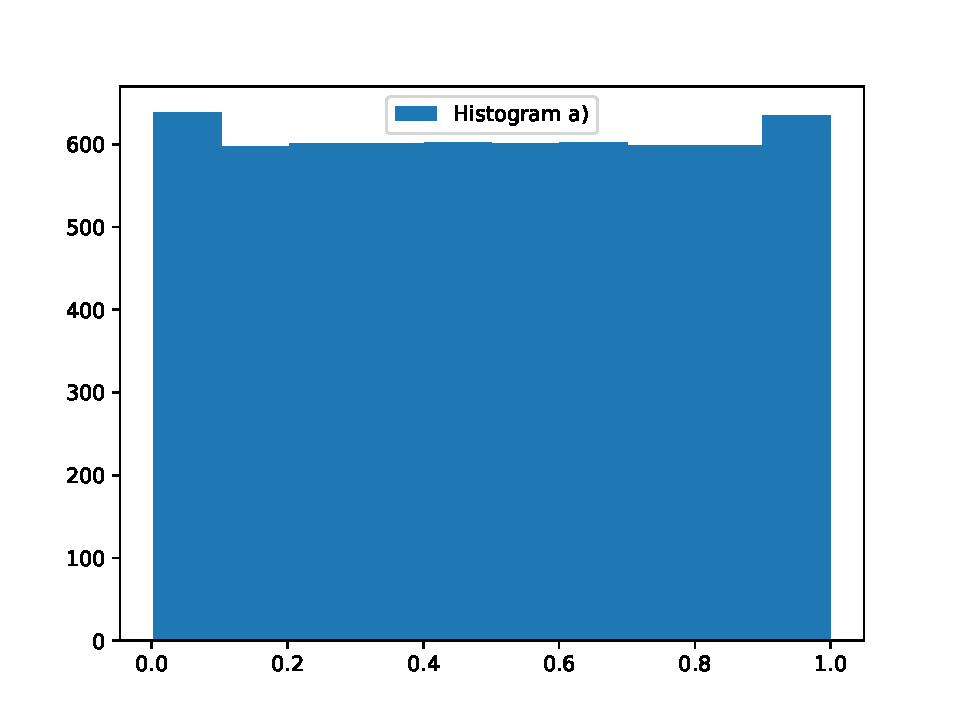
\includegraphics[width=\textwidth]{images/a.pdf}
        \caption{a)}
      \end{subfigure}
      %
      \begin{subfigure}[b]{0.5\textwidth}
        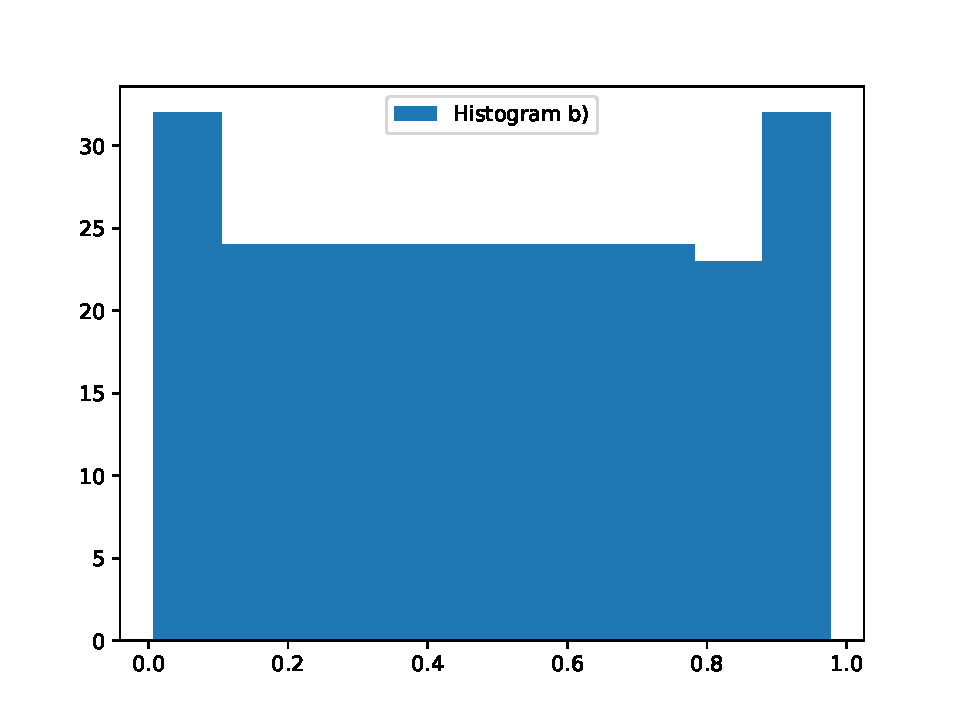
\includegraphics[width=\textwidth]{images/b.pdf}
        \caption{b)}
      \end{subfigure}
      \begin{subfigure}[b]{0.5\textwidth}
        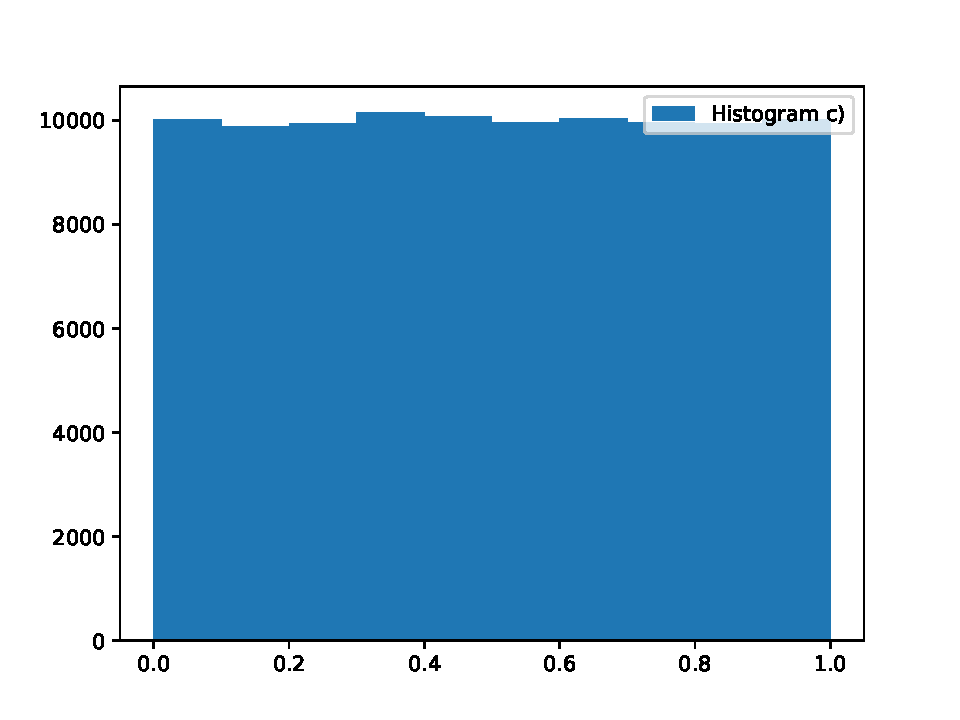
\includegraphics[width=\textwidth]{images/c.pdf}
        \caption{c)}
      \end{subfigure}
      %
      \begin{subfigure}[b]{0.5\textwidth}
        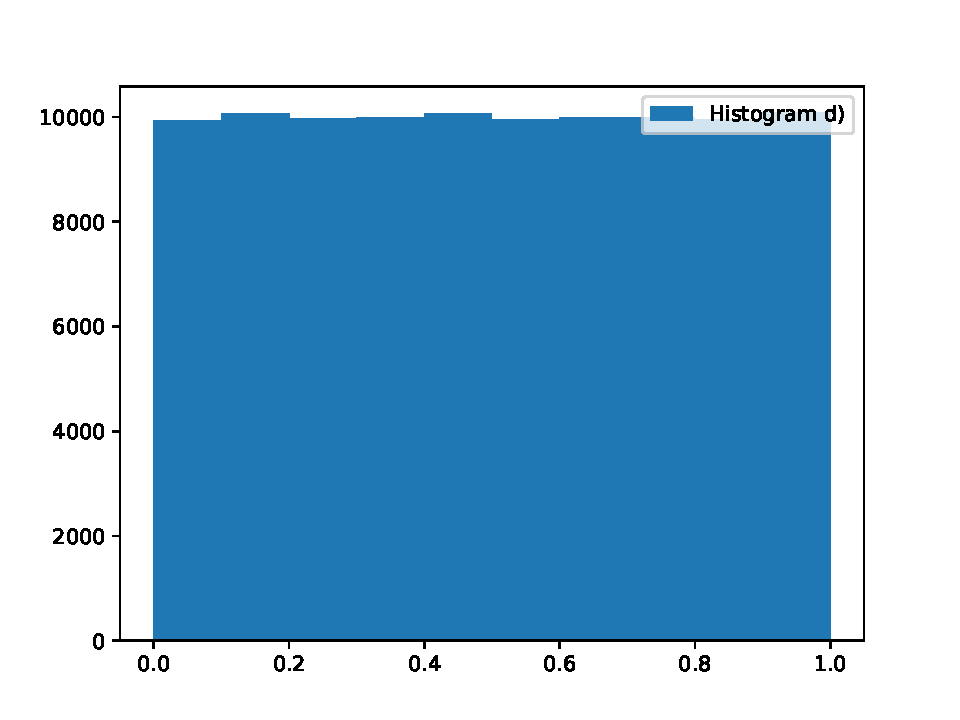
\includegraphics[width=\textwidth]{images/d.pdf}
        \caption{d)}
      \end{subfigure}
      \caption{Histogramme aus 2.}
      \label{fig:2}
    \end{figure}

    3. Die Zufallszahlen werden in Scatterplots aufgetragen. Bei a) und b) lässt sich eine klare Korrelation feststellen. 
    Dies ist ein unerwünschter Nachteil der Linear-Kongruent-Generatoren.
    Bei c) und d) wird nur jedes 10te Wertepaar geplottet, da die Abbildung recht groß ist. Dort ist keine so klare Korrelation zu erkennen.
    Aus der Vorlesung jedoch wissen wir, dass bei einer 3d Darstellung, diese Korrelation klarer zum vorschein kommt.
    

    \begin{figure}
        \begin{subfigure}[b]{0.5\textwidth}
          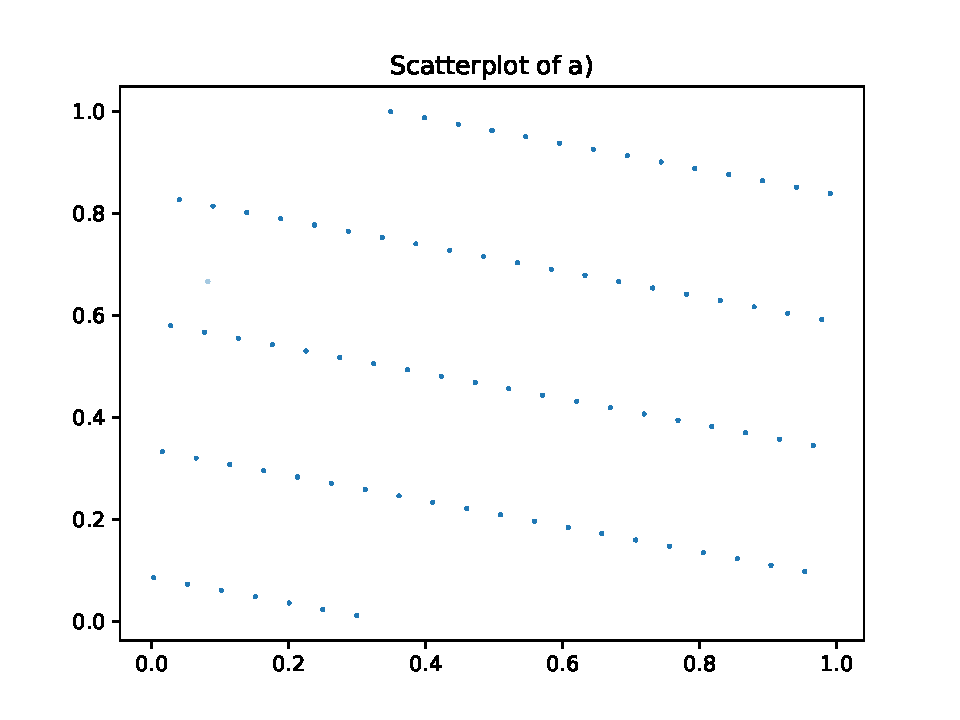
\includegraphics[width=\textwidth]{images/a2d.pdf}
          \caption{a)}
        \end{subfigure}
        %
        \begin{subfigure}[b]{0.5\textwidth}
          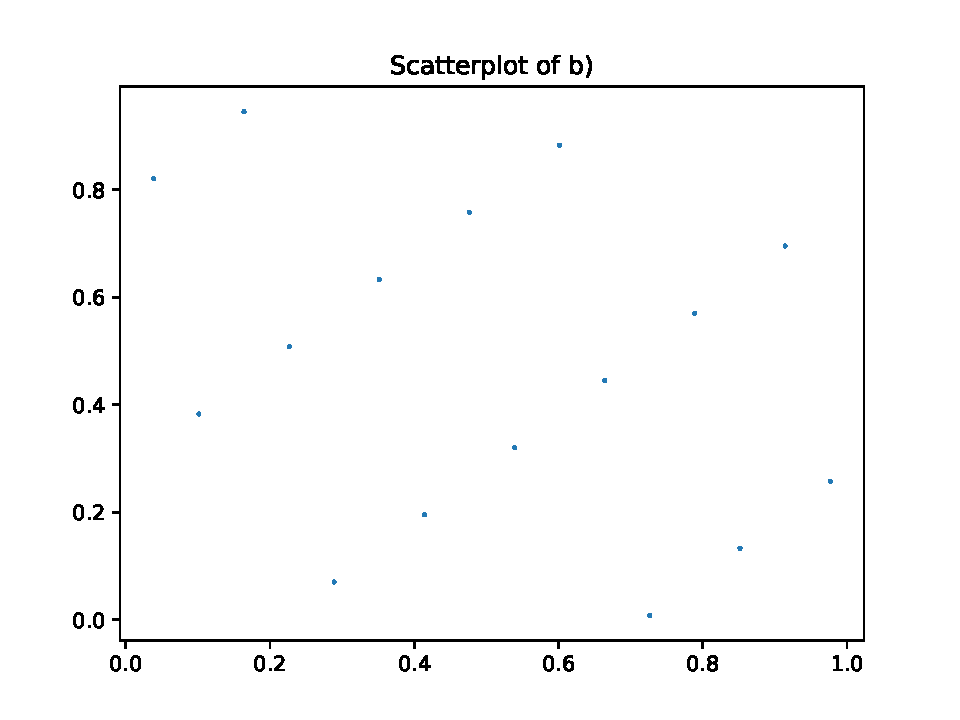
\includegraphics[width=\textwidth]{images/b2d.pdf}
          \caption{b)}
        \end{subfigure}
        \begin{subfigure}[b]{0.5\textwidth}
          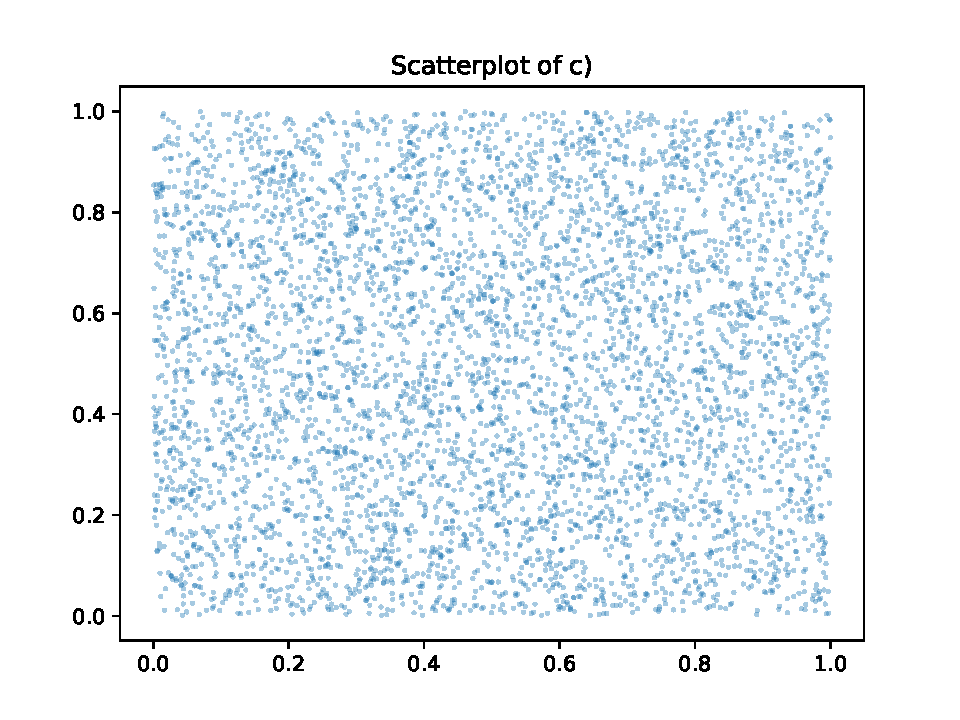
\includegraphics[width=\textwidth]{images/c2d.pdf}
          \caption{c)}
        \end{subfigure}
        %
        \begin{subfigure}[b]{0.5\textwidth}
          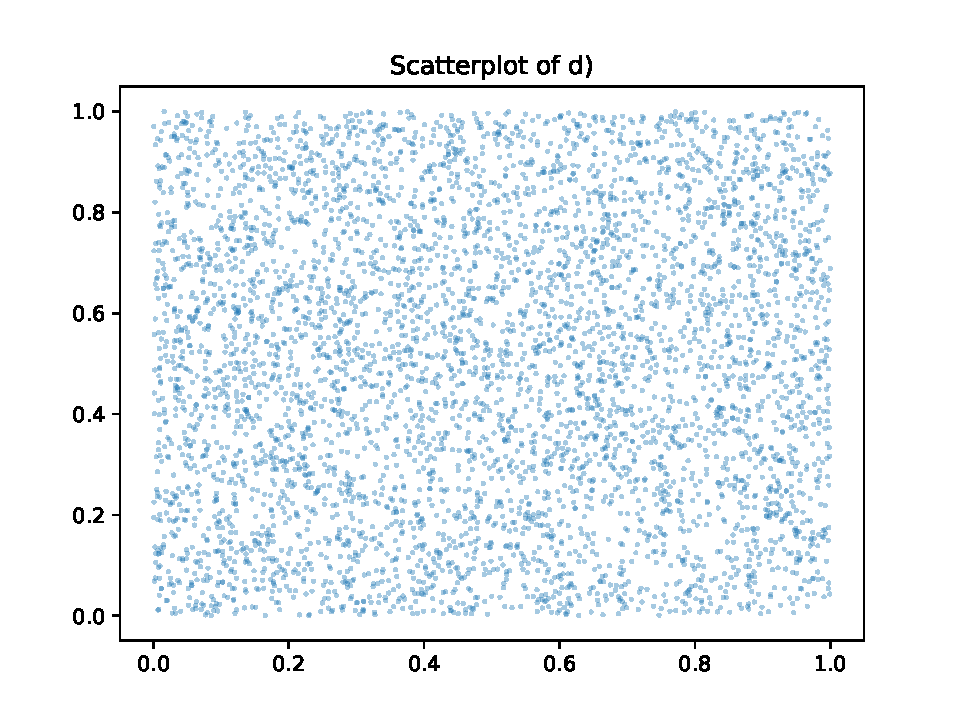
\includegraphics[width=\textwidth]{images/d2d.pdf}
          \caption{d)}
        \end{subfigure}
        \caption{Scatterplots of 3.}
        \label{fig:3}
      \end{figure}


      \subsection{Aufgabe 2}
      \begin{itemize}
        \item[a)]
      Im ersten Teil der Aufgabe sollte der Box-Müller Algorythmus implementriert werden, durch den eine Gauß-verteilung erzeugt wird.
      Wird haben hier den weg über die Darstellung auf einer Kreisschheibe gewählt.
      Wenn der Algorythmus mit $10^5$ Zufallszahlen versogt wird ergibt dieser eine Gaußverteilung, die wir in der folgenden Abbildung dargestellt haben.

      \begin{figure}
        \centering
        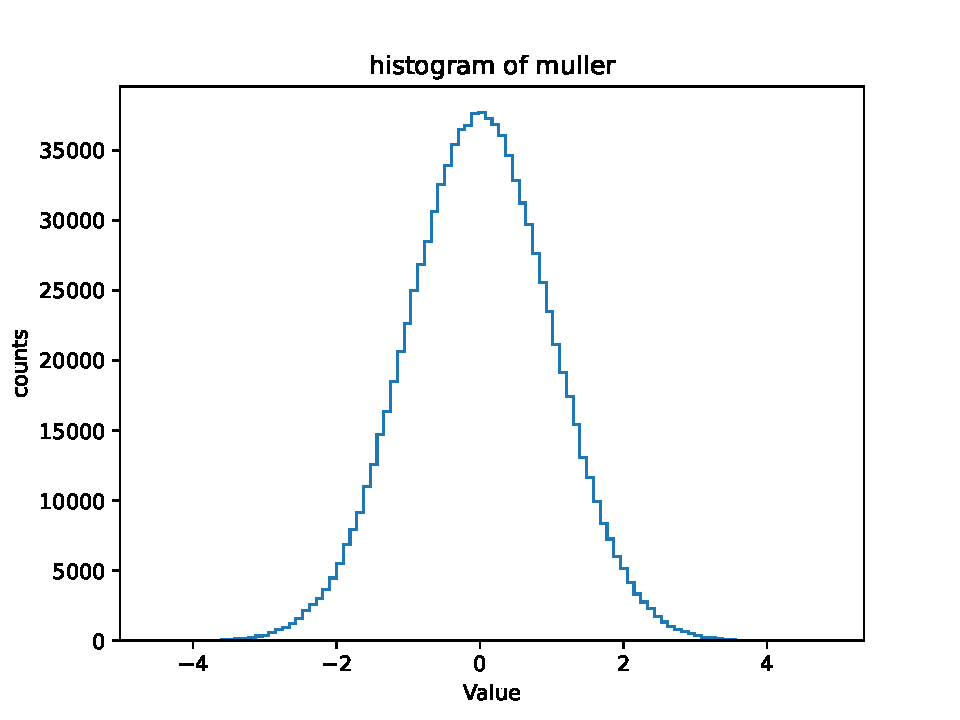
\includegraphics[width=\textwidth]{images/muller_hist.pdf}
        \caption{Der Gaußverteilung welche durch den Box-Müller Algorythmus erstellt worden ist.}
      \end{figure}
      \FloatBarrier
      \item[b)]
      Für den Teil b) der Aufgabe haben wir keine Zeit mehr gehabt, zudem waren wir uns nicht ganz sicher was hier von uns gefragt war.
      \item[c)]
      In Teil c) sollte die Neumann Verwerfungsmethode implementriert werden.
      Diese verwift kurzer Hand alle Werte die nicht zu der gewollten Verteilung passen.
      Dadurch müssen verworfene Zufallszahlen neu gezogen werden, was natürlich bei vielen Zahlen einen stark erhöten Rechenaufwand entspricht.
      Die von uns erstellt implementriert wird an der Funktion 
      \begin{equation}
        p_1 = \frac{sin(x)}{2}
      \end{equation}
      gestestet.
      Das resultat ist in der folgenden Abbildung zu sehen.

      \begin{figure}
        \centering
        \includegraphics[width=\textwidth]{images/rejection.pdf}
        \caption{Der Verwerfungsmethode erzeugt eine Verteilung.}
      \end{figure}
      \FloatBarrier
      \item[d)]
      Die Inversionsmethode hat bei uns nicht geklappt. Die Vorschrift die im Kierfeld script gegeben war kommt uns aber auch etwas komisch vor.
    \end{itemize}
\label{sec:auswertung}
